%%%%%%%%%%%%%%%%%%%%%%%%%%%%%%%%%%%%%%%%%%%%%%%%%%%
%
%  New template code for TAMU Theses and Dissertations starting Fall 2012.  
%  For more info about this template or the 
%  TAMU LaTeX User's Group, see http://www.howdy.me/.
%
%  Author: Wendy Lynn Turner 
%	 Version 1.0 
%  Last updated 8/5/2012
%
%%%%%%%%%%%%%%%%%%%%%%%%%%%%%%%%%%%%%%%%%%%%%%%%%%%
%%%                           SECTION V
%%%%%%%%%%%%%%%%%%%%%%%%%%%%%%%%%%%%%%%%%%%%%%%%%%%
\chapter{\uppercase {FEM Basis Functions for Unstructured Polytopes}}
\label{sec::BF}

%%%%%%%%%%%%%%%%%%%%%%%%%%%%%%%%%%%%%%%%%%%%%%%%%%%
%%%   Section - 2D
\section{Two-Dimensional Basis Functions on Polygons}
\label{sec::BF_2D}


%%%%%%%%%%%%%%%%%%%%%%%%%%%%%%%%%%%%%%%%%%%%%%%%%%%
%%%   SubSection - Linear Basis Functions
\subsection{Linearly-Complete 2D Basis Functions}
\label{sec::BF_2D_Linear}

\begin{equation}
\begin{aligned}
	\sum_{i=1}^{N_K} b_i (\vec{x}) & =  1 \\
	\sum_{i=1}^{N_K} b_i(\vec{x}) \vec{x}_i & =  \vec{x}
\end{aligned}
\label{eq::BF_linear_interp_requirements}
\end{equation}

%%%%%%%%%%%%%%%%%%%%%%%%%%%%%%%%%%%%%%%%%%%%%%%%%%%
%%%   SubSubSection - Linear
\subsubsection{Linear and BiLinear Basis Functions}
\label{sec::BF_2D_Linear_LDandBLD}

Before presenting basis function sets applicable to polytope finite elements, we first provide two basis functions that are exact 

\begin{equation}
\label{eq::2D_lin_basis_functions}
\begin{aligned}
	b_1(r,s) & = 1-r-s \\
	b_2(r,s) & = r \\
	b_3(r,s) & = s 
\end{aligned}
\end{equation}

\noindent 

and

\begin{equation}
\label{eq::BiL_basis_functions}
\begin{aligned}
	b_1(r,s) & = (1-r)(1-s) \\
	b_2(r,s) & = r(1-s) \\
	b_3(r,s) & = rs \\
	b_4(r,s) & = (1-r)s
\end{aligned}
\end{equation}


%%%%%%%%%%%%%%%%%%%%%%%%%%%%%%%%%%%%%%%%%%%%%%%%%%%
%%%   SubSection - Wachspress
\subsubsection{Wachspress Rational Basis Functions}
\label{sec::BF_2D_Linear_Wachspress}

%%%%%%%%%%%%%%%%%%%%%%%%%%%%%%%%%%%%%%%%%%%%%%%%%%%
%%%   SubSection - Mean Value
\subsubsection{Mean Value Basis Functions}
\label{sec::BF_2D_Linear_MV}

%%%%%%%%%%%%%%%%%%%%%%%%%%%%%%%%%%%%%%%%%%%%%%%%%%%
%%%   SubSection - Metric
\subsubsection{Metric Basis Functions}
\label{sec::BF_2D_Linear_Metric}

%%%%%%%%%%%%%%%%%%%%%%%%%%%%%%%%%%%%%%%%%%%%%%%%%%%
%%%   SubSection - Maximum Entropy
\subsubsection{Maximum Entropy Basis Functions}
\label{sec::BF_2D_Linear_ME}

%%%%%%%%%%%%%%%%%%%%%%%%%%%%%%%%%%%%%%%%%%%%%%%%%%%
%%%   SubSection - PWL
\subsubsection{Piecewise Linear (PWL) Basis Functions}
\label{sec::BF_2D_Linear_PWL}

\begin{equation}
\label{eq::PWL_2D}
	b_j (x,y) = t_j (x,y) + \alpha_j^K t_c (x,y)
\end{equation}

\noindent $t_j$ is the standard 2D linear function with unity at vertex $j$ that linearly decreases to zero to the cell center and each adjoining vertex. $t_c$ is the 2D cell ``tent'' function which is unity at the cell center and linearly decreases to zero to each cell vertex. $\alpha_{K,j}$ is the weight parameter for vertex $j$ in cell $K$.

The 3D PWL basis functions share a similar form to the 2D PWL basis functions.

\begin{equation}
\label{eq::PWL_3D}
	b_j (x,y,z)  = t_j  (x,y,z) + \sum_{f=1}^{F_j} \beta_j^f  t_f (x,y,z) + \alpha_j^K t_c  (x,y,z)
\end{equation}

\noindent $t_j$ is the standard 3D linear function with unity at vertex $j$ that linearly decreases to zero to the cell center, the face center for each face that includes vertex $j$, and each vertex that shares an edge with vertex $j$. $t_c$ is the 3D cell ``tent" function which is unity at the cell center and linearly decreases to zero to each cell vertex and face center. $t_f$ is the face "tent" function which is unity at the face center and linearly decreases to zero at each vertex on that face and the cell center. $\beta_{f,j}$ is the weight parameter for face $f$ touching cell vertex $j$, and $F_j$ is the number of faces touching vertex $j$. Like the previous work defining the PWLD method \cite{bailey2008phd}, we also choose to assume the cell and face weighting parameters are

\begin{equation}
\alpha_{K,j} = \frac{1}{N_K} \qquad \text{and} \qquad \beta_{f,j} = \frac{1}{N_f},
\label{eq::PWL_weight_vals}
\end{equation}

\noindent respectively, where $N_K$ is the number of vertices in cell $K$ and $N_f$ is the number of vertices on face $f$, which leads to constant values of $\alpha$ and $\beta$ for each cell and face, respectively. This assumption of the cell weight function holds for both 2D and 3D.

%%%%%%%%%%%%%%%
% Begin::2D PWL basis function plots
\pagebreak
\begin{figure}
\label{fig::2D_PWL_unit_square_basis_functions}
\centering
	\begin{subfigure}[b]{0.48\textwidth}
		\centering
		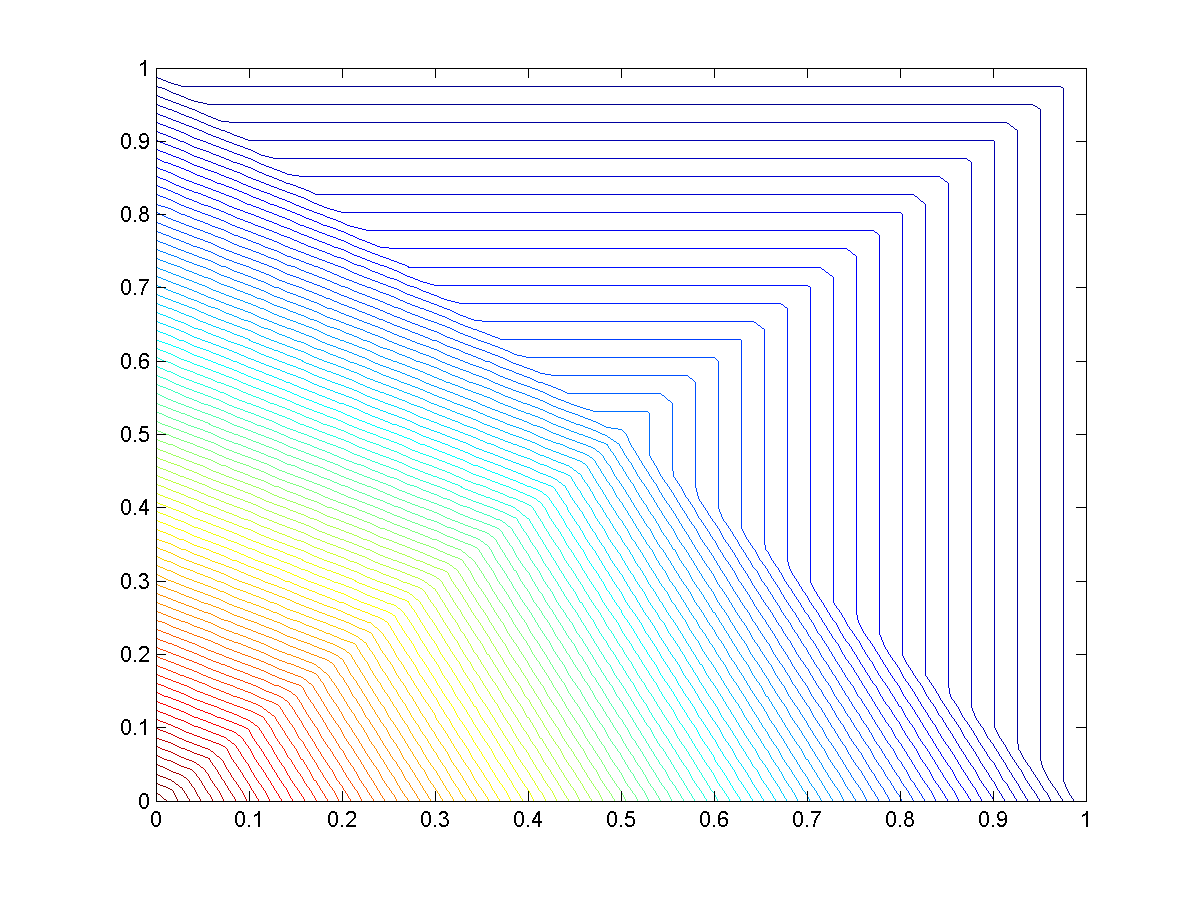
\includegraphics[width=\textwidth]{figures/sec_BF/PWL_square_contour_1.png}
		\caption{}
	\end{subfigure}
	\hfill
	\begin{subfigure}[b]{0.48\textwidth}
		\centering
		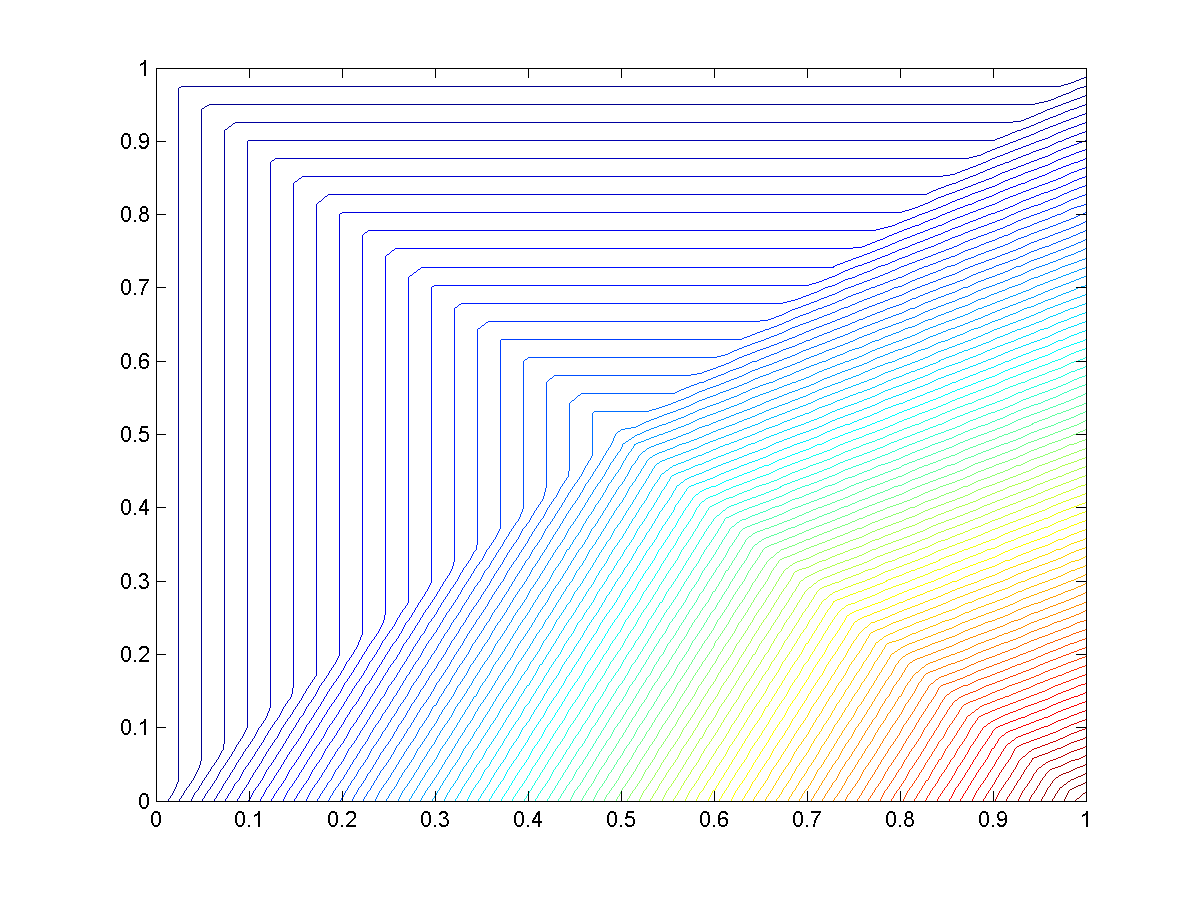
\includegraphics[width=\textwidth]{figures/sec_BF/PWL_square_contour_2.png}
		\caption{}
	\end{subfigure}
	\vfill
	\begin{subfigure}[b]{0.48\textwidth}
		\centering
		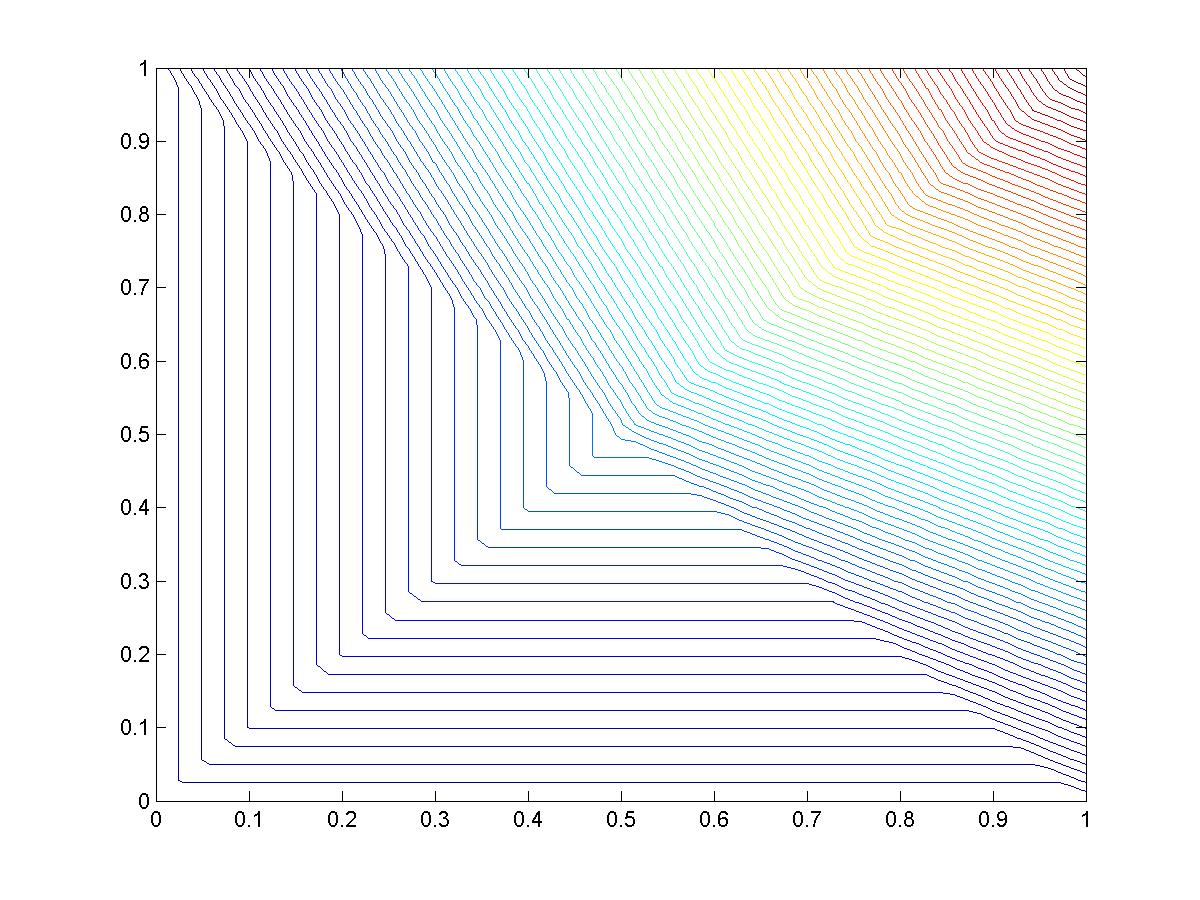
\includegraphics[width=\textwidth]{figures/sec_BF/PWL_square_contour_3.png}
		\caption{}
	\end{subfigure}
	\hfill
	\begin{subfigure}[b]{0.48\textwidth}
		\centering
		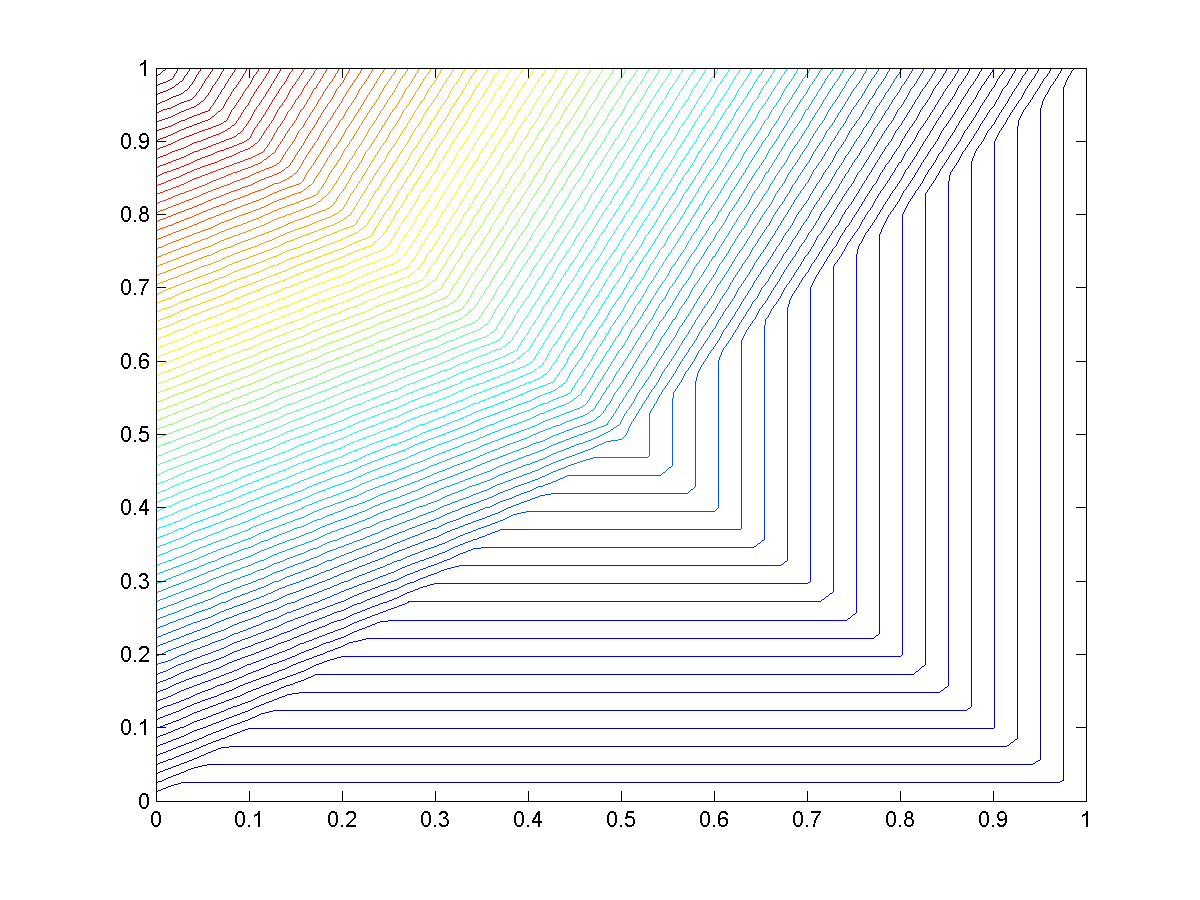
\includegraphics[width=\textwidth]{figures/sec_BF/PWL_square_contour_4.png}
		\caption{}
	\end{subfigure}
\caption{Contour plots of the PWL basis functions on the unit square for the vertices located at: (a) (0,0), (b) (1,0), (c) (1,1), and (d) (0,1).}
\end{figure}

\begin{figure}
\label{fig::2D_pentagon_vertices}
\centering
	\begin{subfigure}[b]{0.40\textwidth}
		\centering
		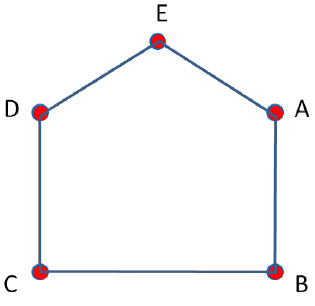
\includegraphics[width=\textwidth]{figures/sec_BF/reg_pent_verts.png}
		\caption{}
	\end{subfigure}
	\hfill
	\begin{subfigure}[b]{0.40\textwidth}
		\centering
		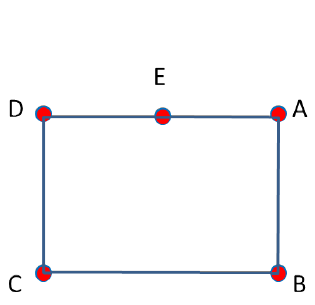
\includegraphics[width=\textwidth]{figures/sec_BF/deg_pent_verts.png}
		\caption{}
	\end{subfigure}
\caption{Vertex structure for a (a) regular pentagonal cell and a (b) degenerate pentagonal cell.}
\end{figure}

\begin{figure}
\label{fig::2D_PWL_pentagon_basis_functions_contour}
\centering
	\begin{subfigure}[b]{0.48\textwidth}
		\centering
		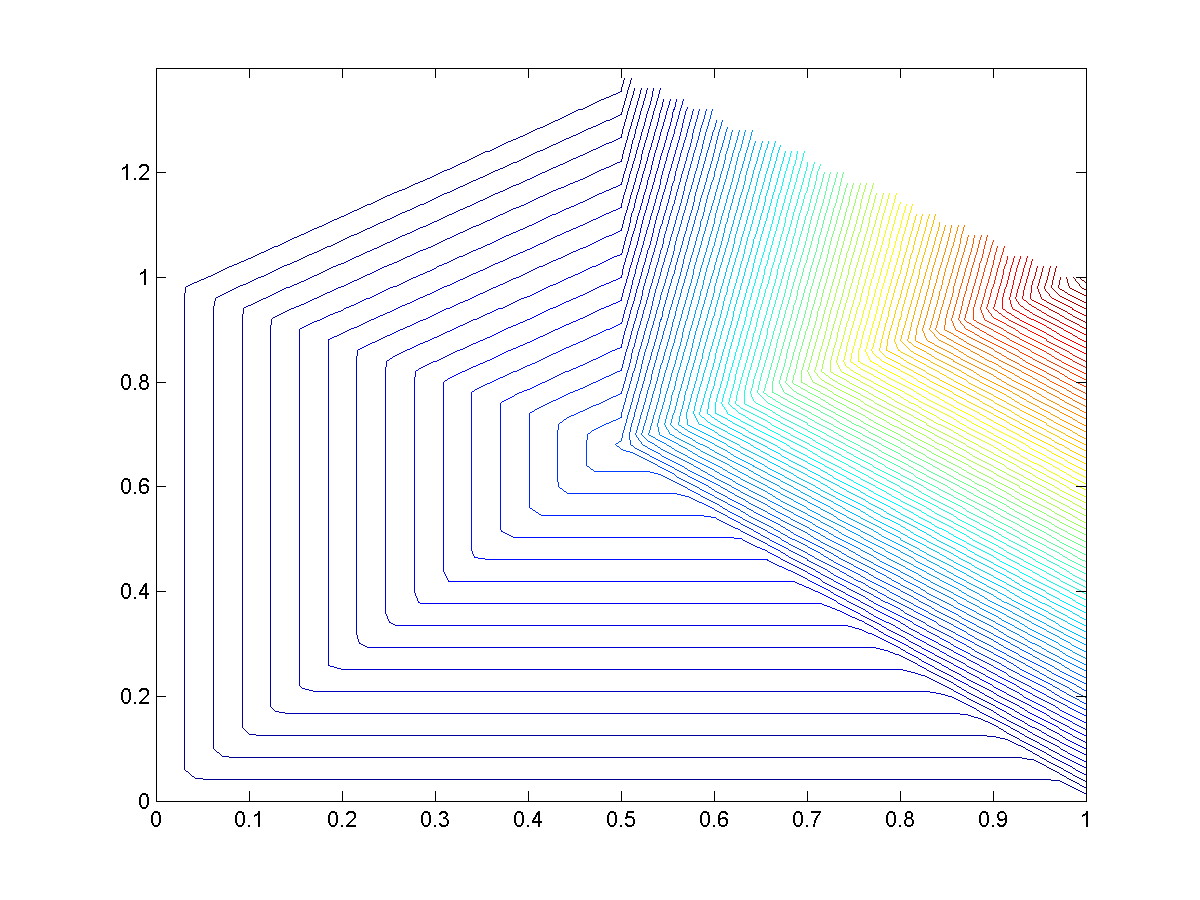
\includegraphics[width=\textwidth]{figures/sec_BF/PWL_rpent_contour_A.png}
		\caption{}
	\end{subfigure}
	\hfill
	\begin{subfigure}[b]{0.48\textwidth}
		\centering
		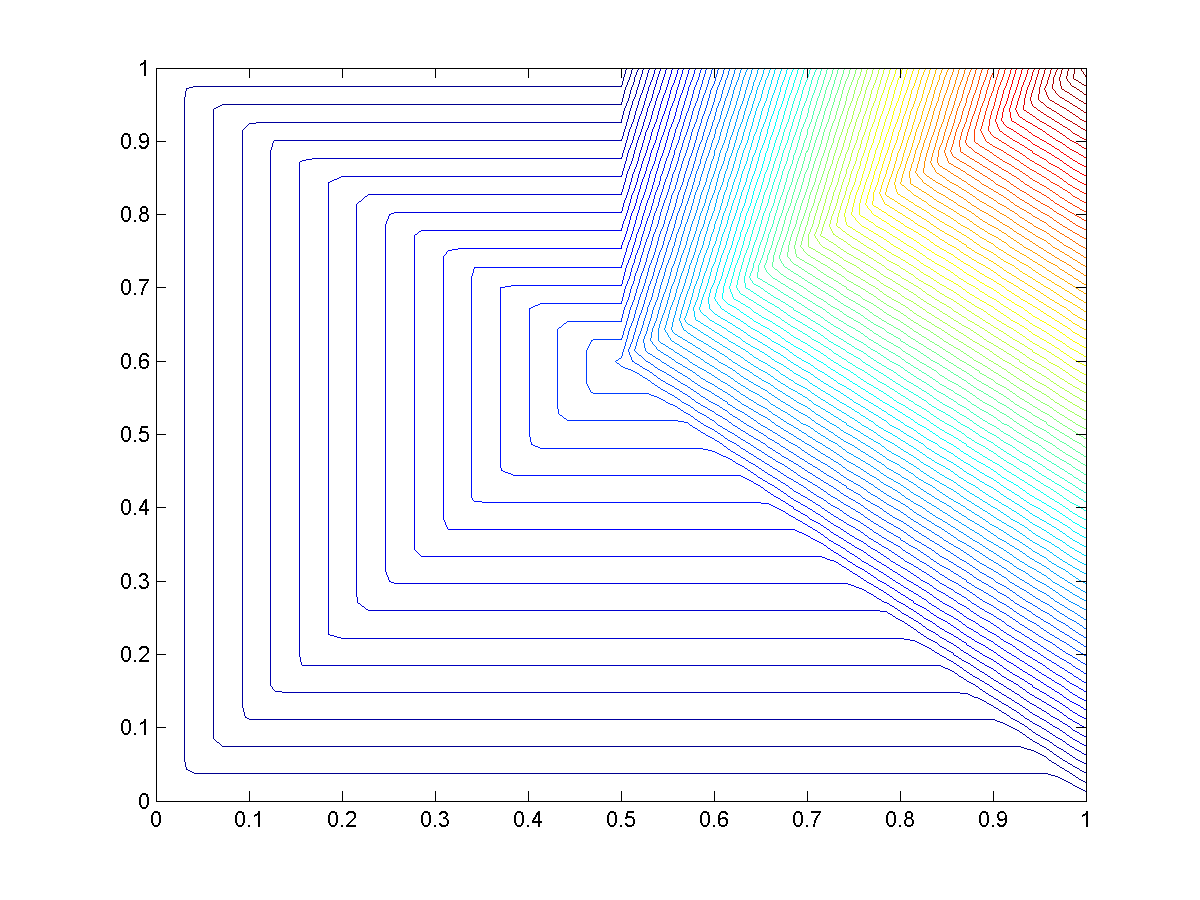
\includegraphics[width=\textwidth]{figures/sec_BF/PWL_dpent_contour_A.png}
		\caption{}
	\end{subfigure}
	\vfill
	\begin{subfigure}[b]{0.48\textwidth}
		\centering
		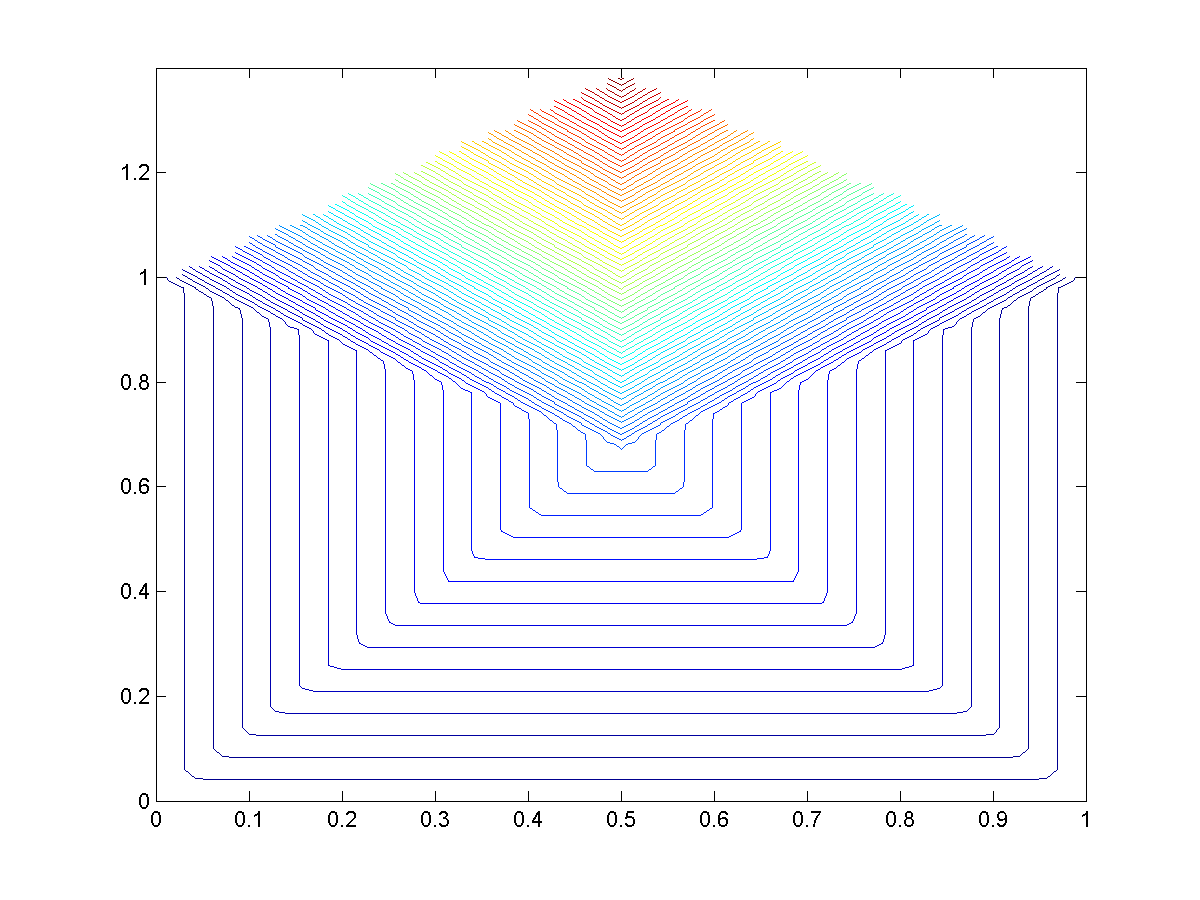
\includegraphics[width=\textwidth]{figures/sec_BF/PWL_rpent_contour_E.png}
		\caption{}
	\end{subfigure}
	\hfill
	\begin{subfigure}[b]{0.48\textwidth}
		\centering
		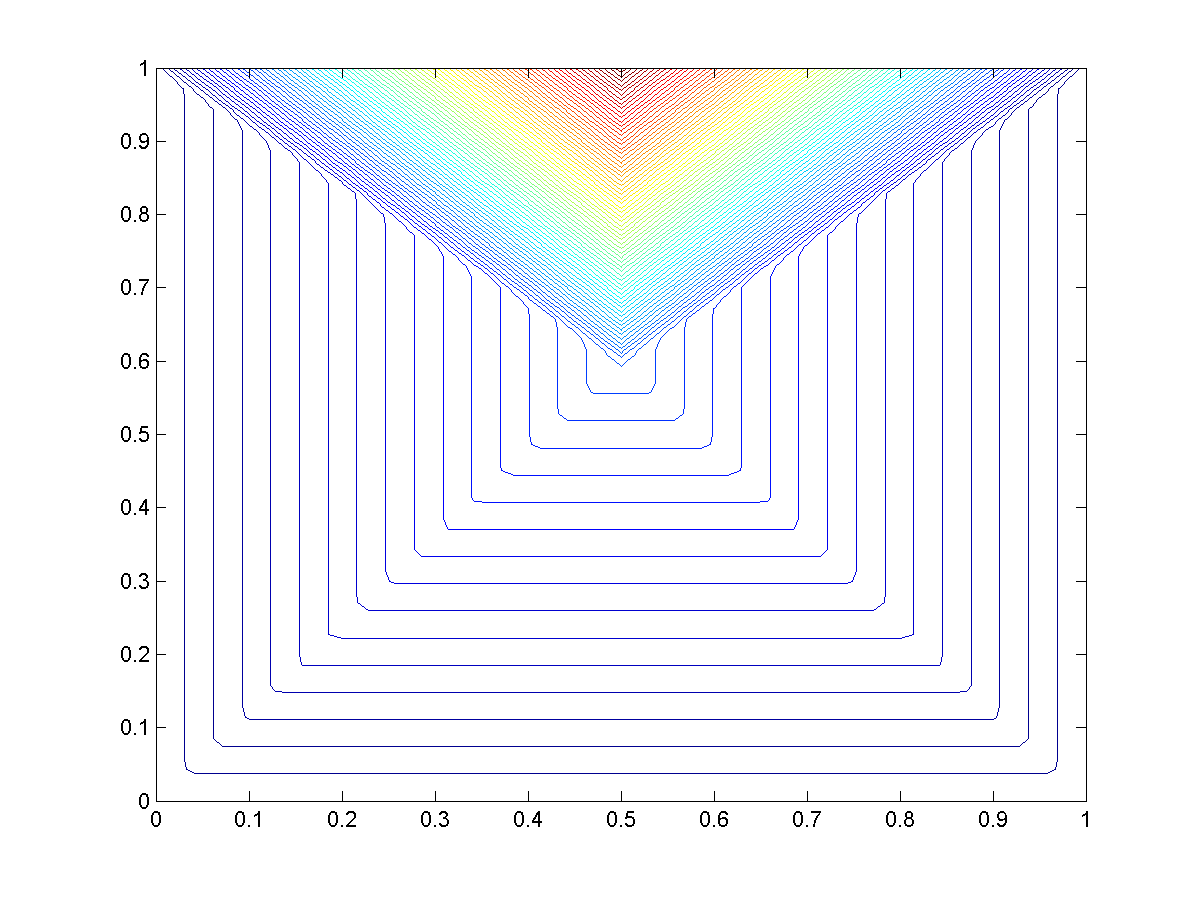
\includegraphics[width=\textwidth]{figures/sec_BF/PWL_dpent_contour_E.png}
		\caption{}
	\end{subfigure}
\caption{Contour plots of the PWL basis functions for a regular pentagon: (a) and (c) as well as a degenerate pentagon: (b) and (d).}
\end{figure}

\begin{figure}
\label{fig::2D_PWL_pentagon_basis_functions_plot}
\centering
	\begin{subfigure}[b]{0.48\textwidth}
		\centering
		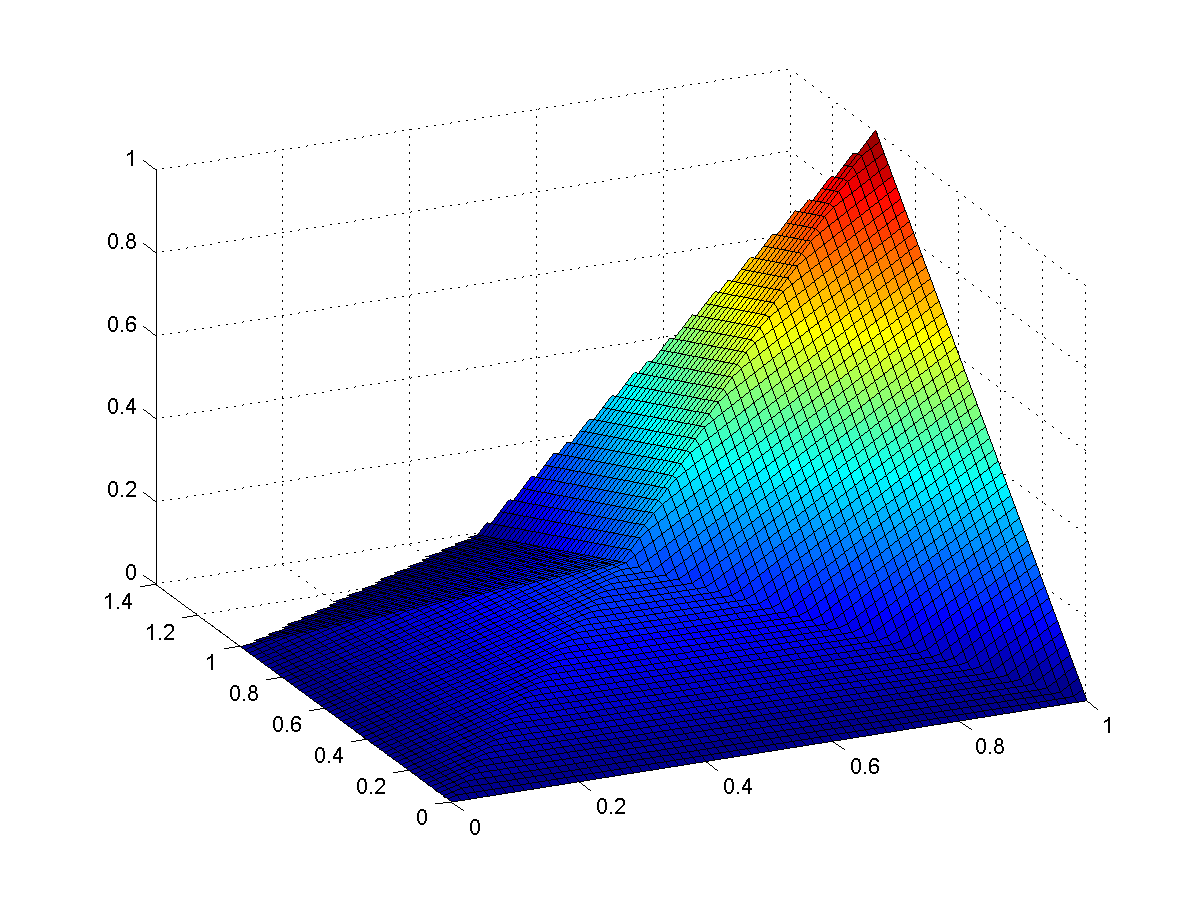
\includegraphics[width=\textwidth]{figures/sec_BF/PWL_rpent_plot_A.png}
		\caption{}
	\end{subfigure}
	\hfill
	\begin{subfigure}[b]{0.48\textwidth}
		\centering
		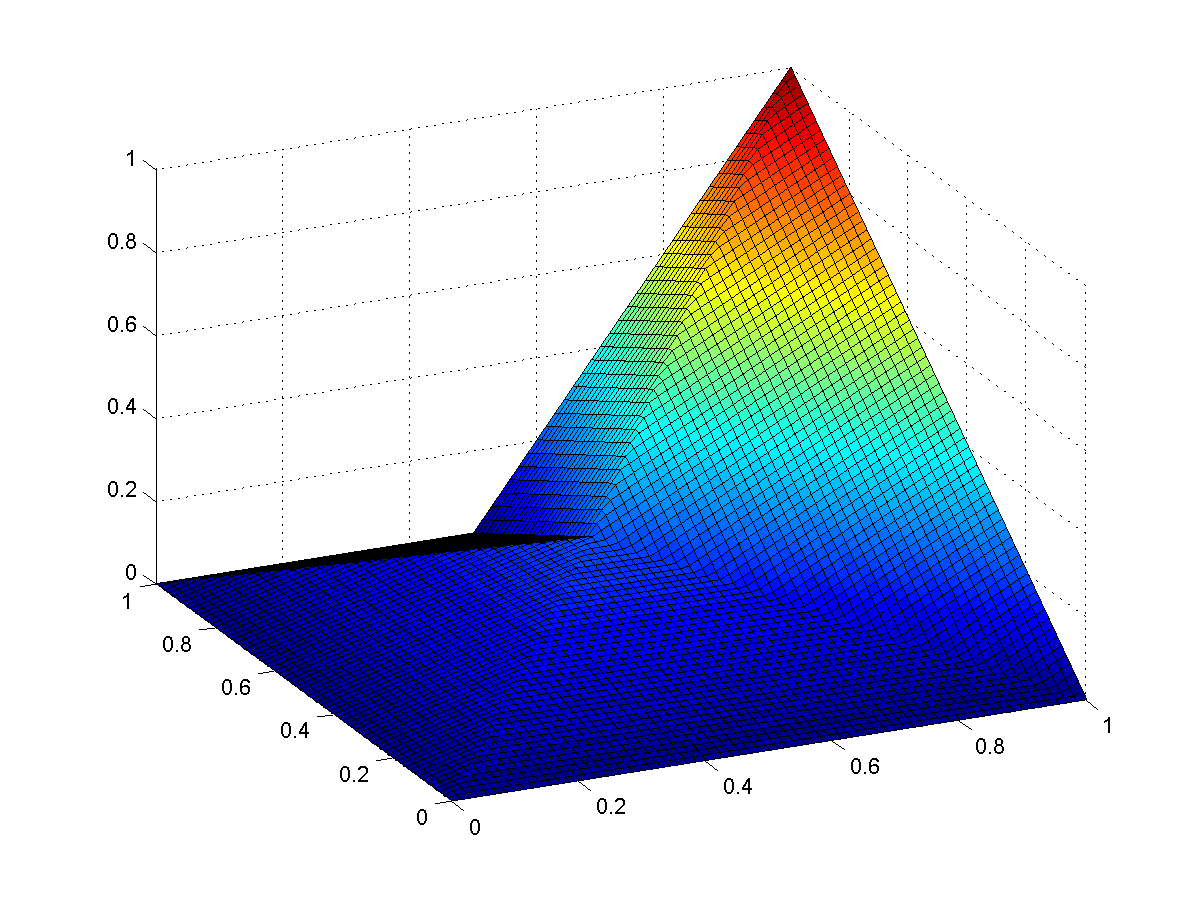
\includegraphics[width=\textwidth]{figures/sec_BF/PWL_dpent_plot_A.png}
		\caption{}
	\end{subfigure}
	\vfill
	\begin{subfigure}[b]{0.48\textwidth}
		\centering
		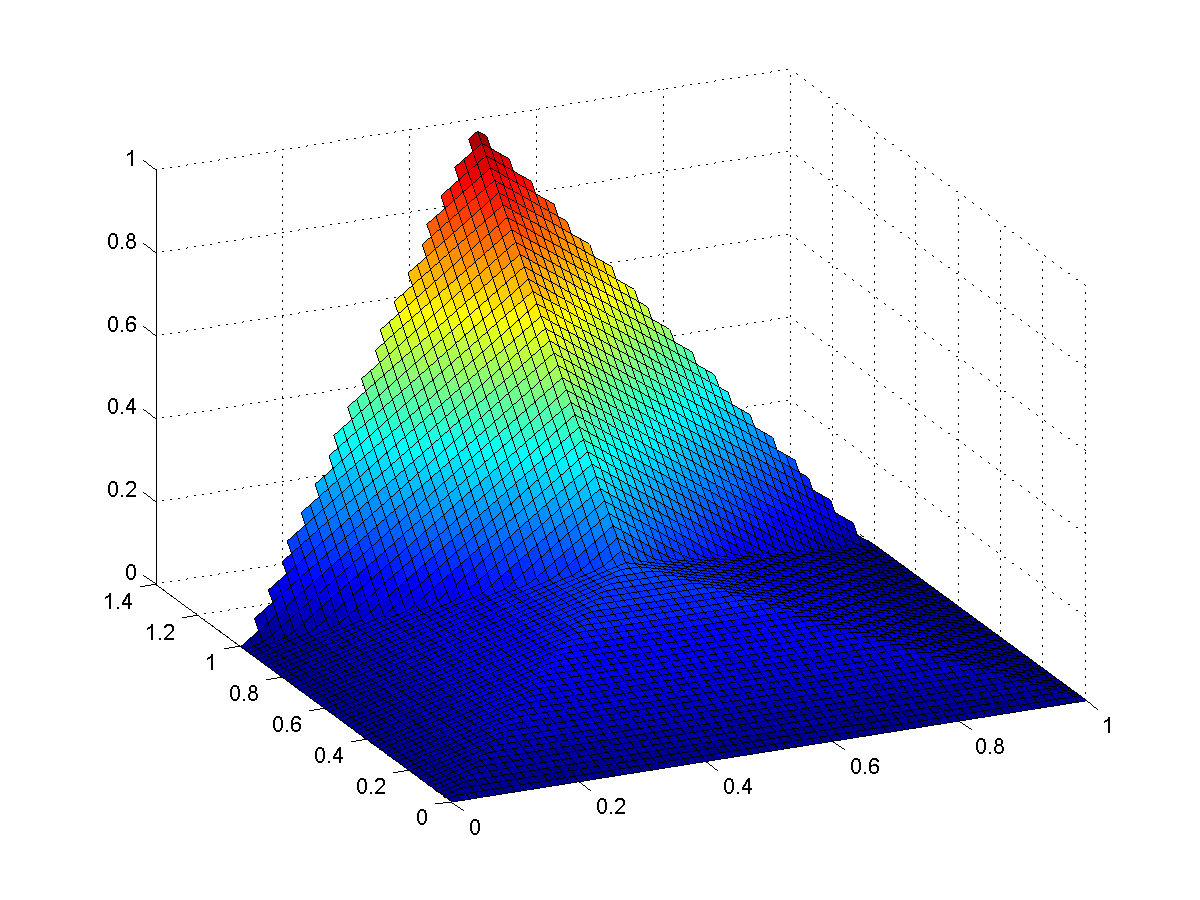
\includegraphics[width=\textwidth]{figures/sec_BF/PWL_rpent_plot_E.png}
		\caption{}
	\end{subfigure}
	\hfill
	\begin{subfigure}[b]{0.48\textwidth}
		\centering
		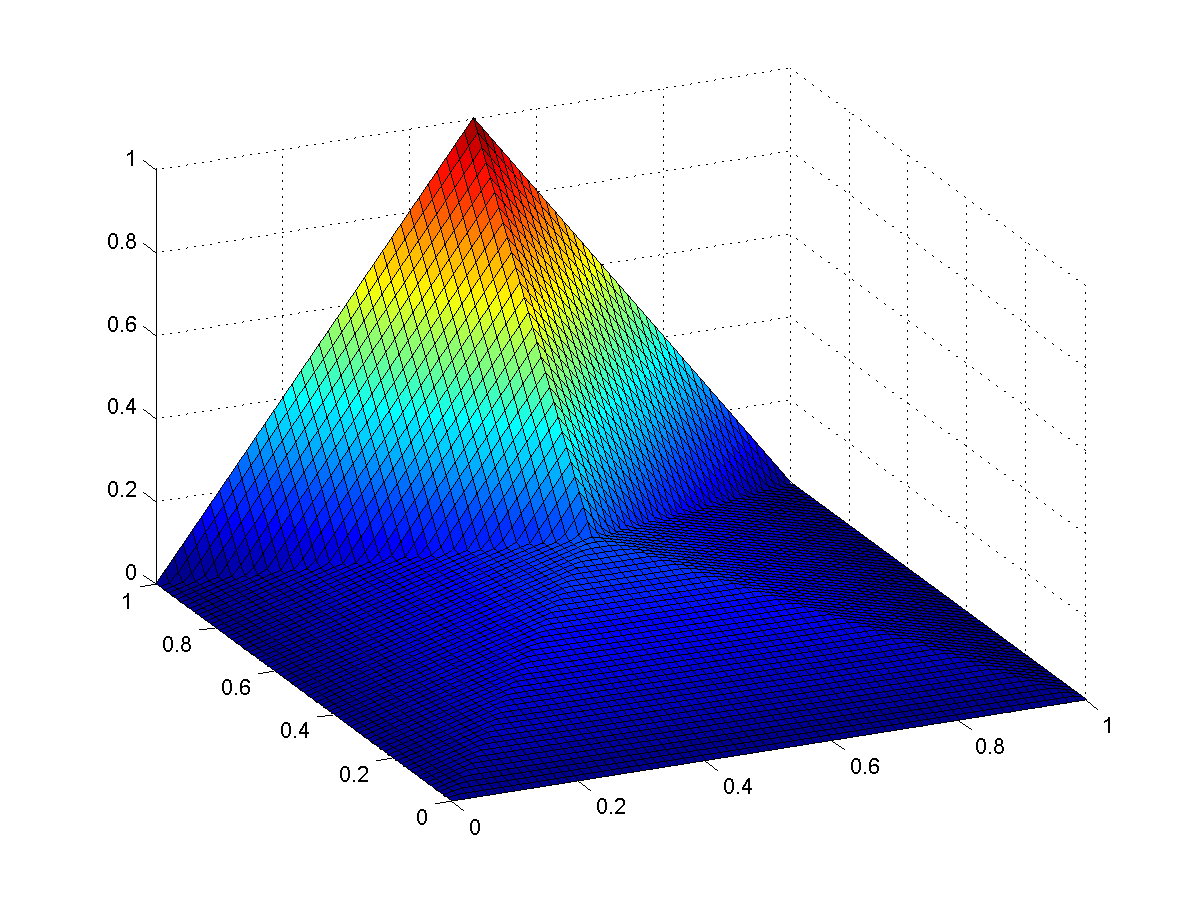
\includegraphics[width=\textwidth]{figures/sec_BF/PWL_dpent_plot_E.png}
		\caption{}
	\end{subfigure}
\caption{Plots of the PWL basis functions for a regular pentagon: (a) and (c) as well as a degenerate pentagon: (b) and (d).}
\end{figure}


% End::2D PWL basis function plots
%%%%%%%%%%%%%%%

%%%%%%%%%%%%%%%%%%%%%%%%%%%%%%%%%%%%%%%%%%%%%%%%%%%
%%%   Section - Quadratic Basis Functions
\subsection{Quadratically-Complete 2D Basis Functions}
\label{sec::BF_2D_Quadratic}

\begin{gather}
	 \sum_{i=1}^{N_K} b_i (\vec{x})  =  1 \\
	\sum_{i=1}^{N_K} b_i(\vec{x}) \vec{x}_i  =  \vec{x} \\
	\sum_{i=1}^{N_K} \sum_{j=1}^{N_K} \mu _{i,j} b_i(\vec{x}) \left(   \frac{\vec{x}_i \otimes \vec{x}_j +\vec{x}_j \otimes \vec{x}_i }{2}  \right)  = \vec{x} \otimes \vec{x}
\label{eq::quadratic_interp_requirements}
\end{gather}

\noindent where $\mu_{i,j}$ is a weight function corresponding to particular basis function pairings.

%%%%%%%%%%%%%%%%%%%%%%%%%%%%%%%%%%%%%%%%%%%%%%%%%%%
%%%   SubSection - BiL/TriL
\subsubsection{Serendipity Bilinear and Trilinear Basis Functions}
\label{sec::BF_Quadratic_BiLTriL}

%%%%%%%%%%%%%%%%%%%%%%%%%%%%%%%%%%%%%%%%%%%%%%%%%%%
%%%   Section - 3D
\section{Three-Dimensional Basis Functions on Polyhedra}
\label{sec::BF_3D}

%%%%%%%%%%%%%%%%%%%%%%%%%%%%%%%%%%%%%%%%%%%%%%%%%%%
%%%   SubSection - 3D Lin/TriL
\subsection{3D Linear and TriLinear Basis Functions}
\label{sec::BF_Linear_BiLTriL}

\begin{figure}
\centering
	\begin{subfigure}[b]{0.45\textwidth}
		\centering
		\label{subfig::unit_square}
		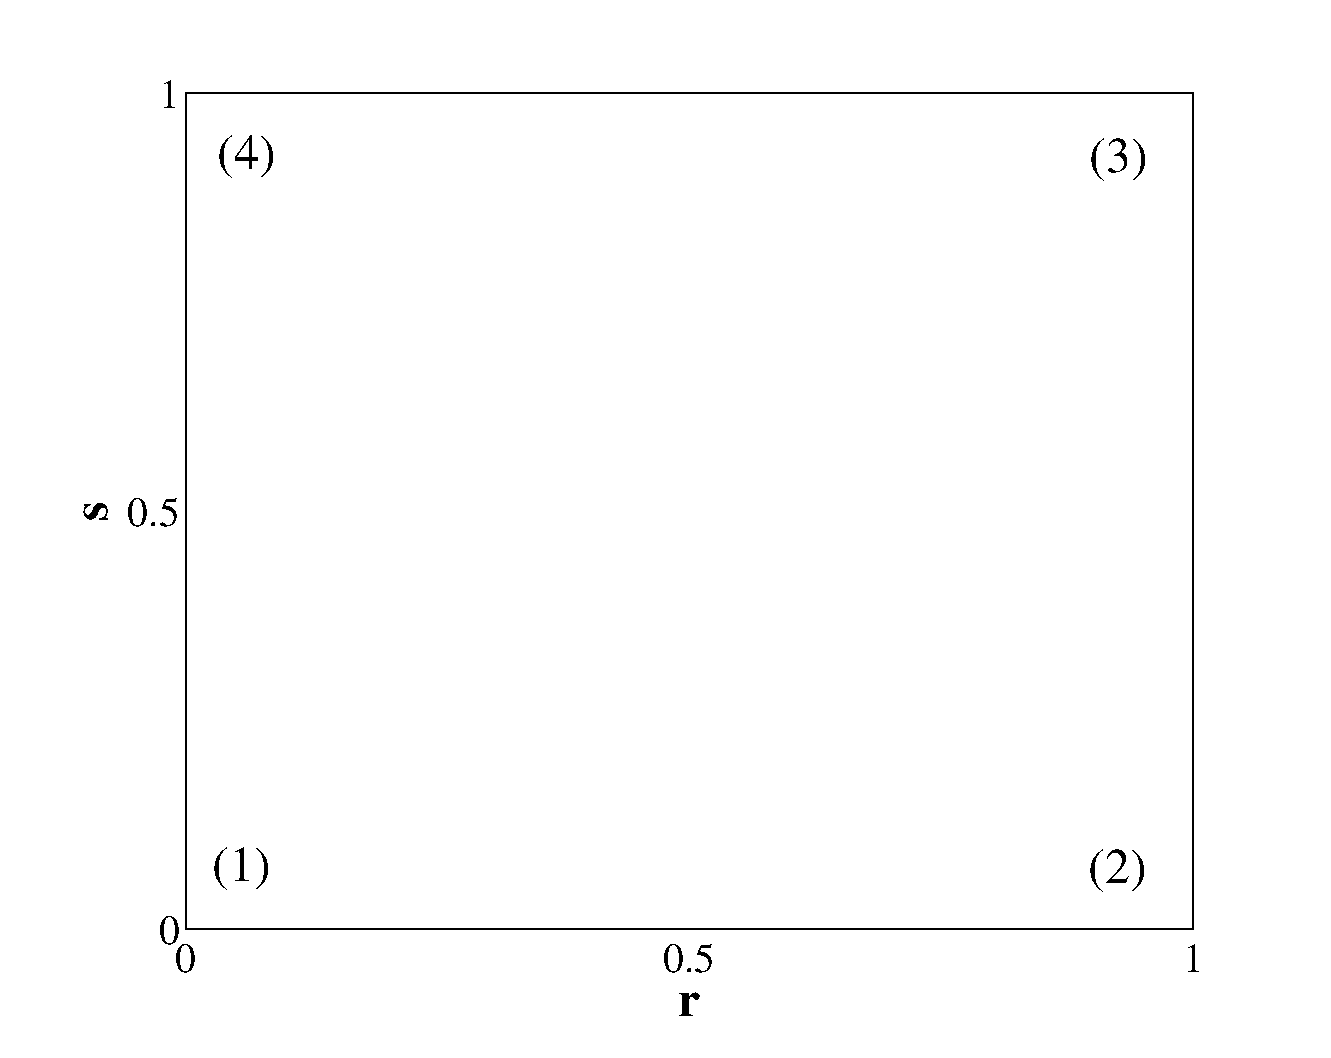
\includegraphics[width=\textwidth]{figures/sec_BF/unit_square_linear.eps}
		\caption{}
	\end{subfigure}
	\hfill
	\begin{subfigure}[b]{0.45\textwidth}
		\centering
		\label{subfig::unit_cube}
		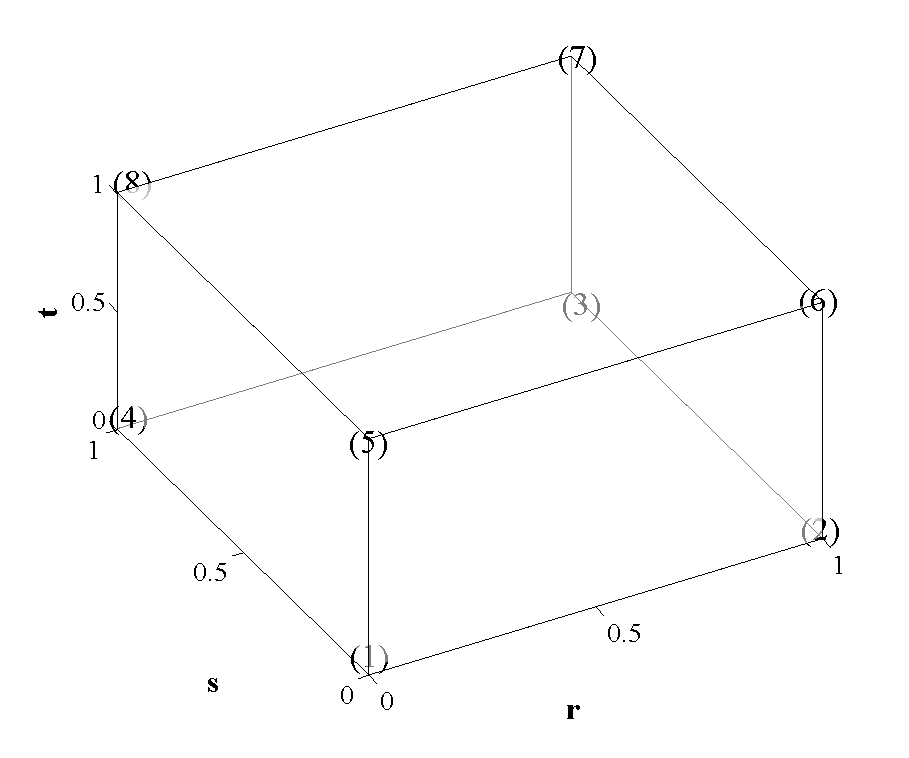
\includegraphics[width=\textwidth]{figures/sec_BF/unit_cube_linear.eps}
		\caption{}
	\end{subfigure}
\caption{Vertex structure for the (a) unit square and (b) unit cube.}
\label{fig::BF_3D_unit_tet_cube}
\end{figure}

\begin{equation}
\label{eq::3D_lin_basis_functions}
\begin{aligned}
	b_1(r,s) & = 1-r-s-t \\
	b_2(r,s) & = r \\
	b_3(r,s) & = s \\
	b_4(r,s) & = t
\end{aligned}
\end{equation}

\noindent and

\begin{equation}
\label{eq::TriL_basis_functions}
\begin{aligned}
	b_1(r,s,t) & = (1-r)(1-s)(1-t) \\
	b_2(r,s,t) & = r(1-s)(1-t) \\
	b_3(r,s,t) & = rs(1-t) \\
	b_4(r,s,t) & = (1-r)s(1-t) \\
	b_5(r,s,t) & = (1-r)(1-s)t \\
	b_6(r,s,t) & = r(1-s)t \\
	b_7(r,s,t) & = rst \\
	b_8(r,s,t) & = (1-r)st \\
\end{aligned}
\end{equation}


%%%%%%%%%%%%%%%%%%%%%%%%%%%%%%%%%%%%%%%%%%%%%%%%%%%
%%%   Section - Conclusions
\section{Conclusions}
\label{sec::BF_Conclusions}









